\chapter{Dynamic Energy Budget model for \textit{Engraulis ringens}}\label{Chap4}

\section{Introduction}\label{Chap4Intro}

Dynamic Energy Budget (DEB) is a biological theory which takes individuals as dynamic systems, considered as the basic level of metabolic organization, relatively easy to make energy and mass balances. This theoretical framework allows us to model the allocation of energy and nutrients in living organisms through its entire life cycle \citep{Kooi2009}, using theoretical assumptions that have remained valid during its 40 years of development \citep{Kooi2020} making it comparable to other approaches in the goal of understanding how an individual and the surrounding environment interact.\\

This theory is particularly popular in ecophysiology and population ecology, where it helps scientists understand how organisms allocate their energy and resources to various life processes, such as growth, maintenance, and reproduction. The DEB theory is based on a set of mathematical equations and concepts that describe how an organism acquires, uses, and allocates energy. These equations take into account factors like energy acquisition (feeding), energy storage, and the trade-offs between various life processes inside the individual. Different individuals (species), present differences that are captured by the DEB theory at the level of their parameter values \citep{Meer2006}. In this way, this theory helps us to understand how a species can flourish or decline, how it competes for resources or how it adapts in different environmental conditions.\\

The strategy is to start from mechanistic considerations at the individual level incorporating details about the physiology of the species defining parameters that describe how the organism acquires, allocates, and uses energy \citep{KooiSabe1986}. These parameters include assimilation rates, growth rates, reproduction rates, maintenance costs, and more, all of which are typically influenced by factors like temperature, food availability, and age, cementing the basic blocks to model studies on \textit{Engraulis ringens} structured population.\\

\textit{E. ringens}, commonly known as the Peruvian anchovy, is a small pelagic fish species found in the southeastern Pacific Ocean along the coasts of South America, particularly in the Humboldt Current system \citep{GutiSwar2007}. Along with the Peruvian anchovy, there is usually an important presence of sardine (\textit{Sardinops sagax}), another small pelagic species, but since the decade of the 2000s, there have been no significant landings off the peruvian coast \citep{CardFran2015}, and the fact that \textit{E. ringens} is usually associated with the coastal zone while sardines occupy more oceanic areas due to different feeding and oxygen conditions \citep{EspiBert2008,BertChai2011}, we can study the interaction of anchovy with their environment without considering a competition with sardines.\\

When commercially targeted marine fish feed on phytoplankton and zooplankton, they assimilate and redistribute essential nutrients, influencing the productivity and structure of the ecosystem \citep{LeMeGuie2022}. Also, anchovies help maintain the balance and stability of marine ecosystems due their population dynamics can impact the abundance of other species, influencing ecosystem health and resilience to environmental changes \citep{FennSear2023}. Since Dynamic Energy Budget theory can be used in IBM models, ecosystem models, toxicology models \citep{LavaFilg2021}, a DEB model for \textit{E. ringens} is essential for future ecological studies and for conservation purposes.

Below, we list some important concepts in DEB modelling:

\begin{itemize}
%  \centering
  \item Energy Budget: DEB modeling starts by quantifying the energy fluxes into and out of an organism. This includes energy gained through feeding, losses due to metabolism and maintenance, growth, reproduction, and other processes.\\
  
  \item Allocation and Utilization: The model describes how the acquired energy is allocated and utilized for different biological processes, such as growth, reproduction, and maintenance. It helps to understand how organisms prioritize energy allocation under varying conditions.\\

  \item Reserves and Structure: DEB models account for the storage of surplus energy as reserves (e.g., fat, proteins) and the development of structural components (e.g., organs, tissues). The dynamics of these reserves are critical in understanding an organism's life history.\\

  \item Maintenance and Maturation: DEB models consider the energy spent on maintaining basic bodily functions (maintenance) and the energy used for growth and development (maturation) at different life stages.\\

  \item Environmental Factors: The model incorporates two principal environmental factors like temperature, food availability, and other abiotic factors (not taken into account in this study) to assess their influence on energy acquisition, utilization, and allocation.\\

\end{itemize}

In addition, we present a list of potential uses of a DEB model:

\begin{itemize}
%  \centering
  \item Growth and Development: DEB models provide insights into the growth patterns and development stages of organisms. They help predict how growth rates vary with environmental conditions and resource availability.\\
  
  \item Reproduction and Life History Strategies: DEB models enable the study of reproductive strategies, including the timing and allocation of energy to reproduction. This aids in understanding reproductive trade-offs and strategies for optimizing its survival.\\
  
  \item 	Responses to Environmental Change: DEB models help predict how organisms respond to changes in environmental conditions, such as temperature, nutrient availability, and pollution. This is crucial for assessing the impacts of climate change and other environmental stressors.\\
  
  \item Optimizing Fisheries and Aquaculture: DEB models aid in optimizing fisheries and aquaculture practices by predicting growth rates, maturation, and reproduction, leading to sustainable management of fish stocks.\\
  
  \item Toxicology and Ecotoxicology: Although it is not the objective of this study, DEB models can be applied to assess the effects of toxins and pollutants on an organism's energy allocation and life history traits, aiding in understanding toxicological impacts.\\

\end{itemize}

So, in this chapter, we will start by showing the available data collection, the calibration of a DEB model with growth acceleration during its early life stages (that was not taken into account in the Chapter \ref{Chap3}) and its implementation in the IBM called Ichthyop-DEB model, to explore the interaction of the species with its environment, focusing mainly on its food demand since the effect of temperature has been well documented previously.

\section{Methods}\label{Chap4Meth}

\subsection{Data collection}\label{Chap4MethDat}

A model is composed of mathematical equations that represent the characteristics of a dynamic system. These equations include parameters that allow the comparison of different systems, and these parameters are estimated from empirical data \citep{RaolGiri2004}. Gather empirical data and literature data related to \textit{E. ringens}, includes growth rates, especially in their early stages of life, reproduction rates, feeding rates, body sizes, and any other relevant biological measurements.\\

In spite of the application of DEB theory is challenging because the state variables and parameters are abstract quantities that are not directly observable, the parameter estimation method \citep{Lika2011a,Lika2011b} makes use of different data sources.\\

However, there are different levels of difficulty in collecting individual or population data for a species. For example, a collection of population data for \textit{E. ringens} is well described by \citep{MarzShin2009}, but data on metabolic rates, feeding rates or vertical behaviour (characteristics that require captive breeding) have been studied more in other similar species and other ecosystems \citep{AldaCota2008,CermUria2003,KramZwei1968,DetwHoud1970,Hunt1971,Hunt1984,SakaKimu1976,Houd1977,MethKram1979,Thei1980,Brow1983}, while laboratory rearing (especially for early life stages) is just beginning for \textit{E. ringens} \citep{RiouOfel2021,OfelMoya2023}, difficulty in rearing, which can be explained by the high migratory behaviour of anchovies in general \citep{OlivSala2001,MoraBaba2010,TanaOhsh2010,PoliHure2015,GuraFach2017,CastNiqu2021}.\\

The following is a description of the available and preferably most updated data used for DEB parameters estimation on \textit{E. ringens}.\\

\subsection{Parameter estimation}

Estimating parameters for a Dynamic Energy Budget (DEB) model involves a process to fit the model to empirical data, allowing it to accurately represent the energy allocation and life history of a specific organism, in this case, \textit{E. ringens}.\\

We used a bivariate statistical technique \citep{Lika2011a,Lika2011b} to estimate the values of the model parameters that minimize the difference between model predictions and observed data. Then, we fitted the DEB model to the compiled empirical data, adjusting parameters to best represent the biological processes and energy dynamics of \textit{E. ringens}.\\

In order to show the difference between the DEB-standard model (\textit{E. encracicolus}) used in Chapter \ref{Chap3}, a comparative table with the estimated parameters for \textit{E. ringens} is presented below.

Table 1: Parameters used for the bioenergetic model describing larval growth. These values were estimated by Pethybridge et al. (2013) for Engraulis encrasicolus and compared with the parameters estimated for E. ringens (current study). The values of $T_L$, $T_H$, $T_AL$, $T_AH$ are detailed for case 1. Values for case 2 are indicated in parenthesis when different from case 1.

\begin{figure}[ht]
	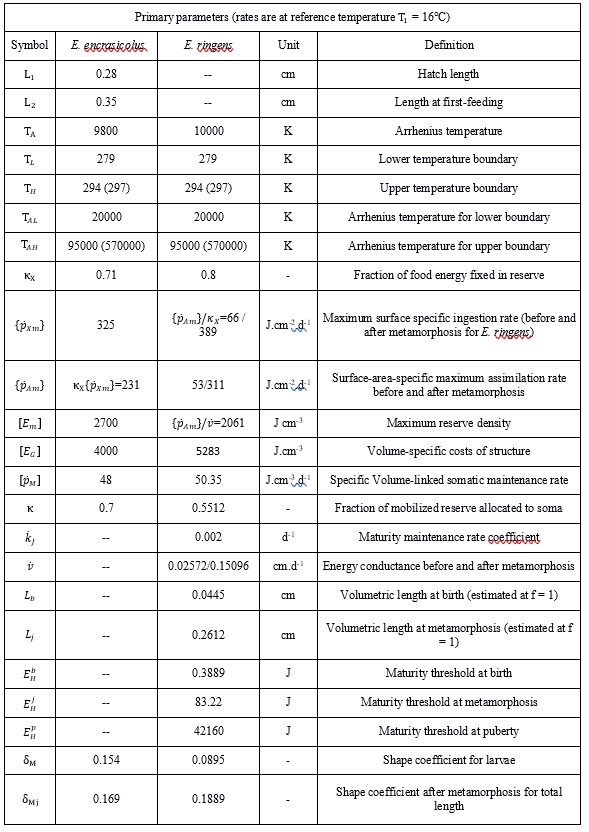
\includegraphics[width=1.0\textwidth]{figures/tablepars.png}
	\centering
	%\caption{Temperature correction curves for the metabolic flux in the dynamic energy budget model \textcolor{red}{(equation 5), revisar la ref cruzada}; blue and red curve correspond respectively to case 1 and case 2 in Table 1.}
%	\label{Fig3_02}
\end{figure}

%\begin{table}[]
%\begin{tabular}{lllll}
%\multicolumn{5}{l}{\textbf{Primary parameters (rates are at reference temperature T\_1 = 16°C)}} \\
%\textbf{Symbol} &
%  \textbf{\textit{E. encrasicolus}} &
%  \textbf{\textit{E. ringens}} &
%  \textbf{Unit} &
%  \textbf{Definition} \\
%L\_1                    & 0.28           & --                    & cm     & Hatch length                                            \\
%L\_2                    & 0.35           & --                    & cm     & Length at first-feeding                                 \\
%T\_A                    & 9800           & 10000                 & K      & Arrhenius temperature                                   \\
%T\_L                    & 279            & 279                   & K      & Lower temperature boundary                              \\
%T\_H                    & 294 (297)      & 294 (297)             & K      & Upper temperature boundary                              \\
%T\_AL                   & 20000          & 20000                 & K      & Arrhenius temperature for lower boundary                \\
%T\_AH                   & 95000 (570000) & 95000 (570000)        & K      & Arrhenius temperature for upper boundary                \\
%κ\_X                    & 0.71           & 0.8                   & -      & Fraction of food energy fixed in reserve                \\
%\{p ̇\_Xm \} &
%  325 &
%  \{p ̇\_Am \}/κ\_X=66 / 389 &
%  J.cm-2.d-1 &
%  Maximum surface specific ingestion rate (before and after metamorphosis for E. ringens) \\
%\{p ̇\_Am \} &
%  κ\_X \{p ̇\_Xm \}=231 &
%  53/311 &
%  J.cm-2.d-1 &
%  Surface-area-specific maximum assimilation rate before and after metamorphosis \\
%{[}E\_m {]}             & 2700           & \{p ̇\_Am \}/v ̇=2061 & J cm-3 & Maximum reserve density                                 \\
%{[}E\_G {]}             & 4000           & 5283                  & J.cm-3 & Volume-specific costs of structure                      \\
%κ                       & 0.7            & 0.5512                & -      & Fraction of mobilized reserve allocated to soma         \\
%k ̇\_J                  & --             & 0.002                 & d-1    & Maturity maintenance rate coefficient                   \\
%v ̇                     & --             & 0.02572/0.15096       & cm.d-1 & Energy conductance before and after metamorphosis       \\
%L\_b                    & --             & 0.0445                & cm     & Volumetric length at birth (estimated at f = 1)         \\
%L\_j                    & --             & 0.2612                & cm     & Volumetric length at metamorphosis (estimated at f = 1) \\
%E\_H\textasciicircum{}b & --             & 0.3889                & J      & Maturity threshold at birth                             \\
%E\_H\textasciicircum{}j & --             & 83.22                 & J      & Maturity threshold at metamorphosis                     \\
%E\_H\textasciicircum{}p & --             & 42160                 & J      & Maturity threshold at puberty                           \\
%δ\_M                    & 0.154          & 0.0895                & -      & Shape coefficient for larvae                            \\
%δ\_Mj                   & 0.169          & 0.1889                & -      & Shape coefficient after metamorphosis for total length  \\
%                        &                &                       &        &                                                        
%\end{tabular}
%\end{table}

